%%%%%%%%%%%%%%%%%%%%%%%%%%%%%%%%%%%%%%%%%%%%%%%%%%%%%%%%%%%%%%%%%%%%%%%%%%%%%
\section{GPGPU Introduction}

GPGPU (\textit{General Purpose computation on Graphics Processor Unit}), also known as \textit{GPU Computing}, is the utilization of the graphic adapter of a personal computer to perform generic and non-graphic related computation that is usually handled by the CPU.\\
Once designed and optimized specifically to perform only fixed graphic calculations, modern GPUs are evolving into \emph{high-performances many-core} processors that can be virtually used to perform any task, and developers who port their applications to GPUs are able to achieve speedups of orders of magnitude vs. optimized CPU implementations of the same code.\cite{GPGPUORG:About}\\
The reason why GPUs are so fast has to be searched in the nature of what graphic rendering is about, that is an \emph{intensive parallel computation}: GPUs are engineered to work specifically on \emph{parallel data processing}, rather than data caching, flow control and pipelined execution like CPUs. (\textbf{Figure \ref{fig:cpuvsgpu_scheme}})

\begin{figurehere}
 \centering
 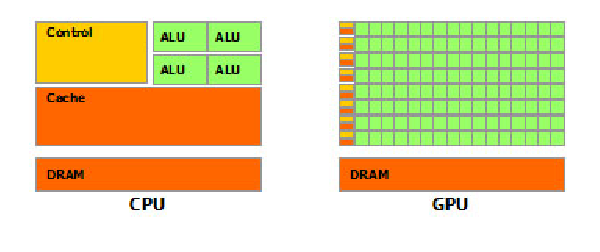
\includegraphics[width=8cm, height=4cm]{./eps/GPU_CPU_struct.eps}
 \caption{GPUs are more focused to computation rather than data caching.}
 \label{fig:cpuvsgpu_scheme}
\end{figurehere}

Moreover, computational units of GPUs are smaller and more numerous (typical GPUs can host hundreds of cores, while CPUs usually contains only 2 or 4) and are highly specialized to perform simple operation \emph{in parallel} over a huge amount of data at the same time.\\
GPUs have been built to exploit application parallelism, and their particular architecture allow them to execute up to a couple TeraFlops of operations per second, against to the few GigaFlops that a single CPU can handle alone. (\textbf{Figure \ref{fig:cpuvsgpu}})

\begin{figurehere}
 \centering
 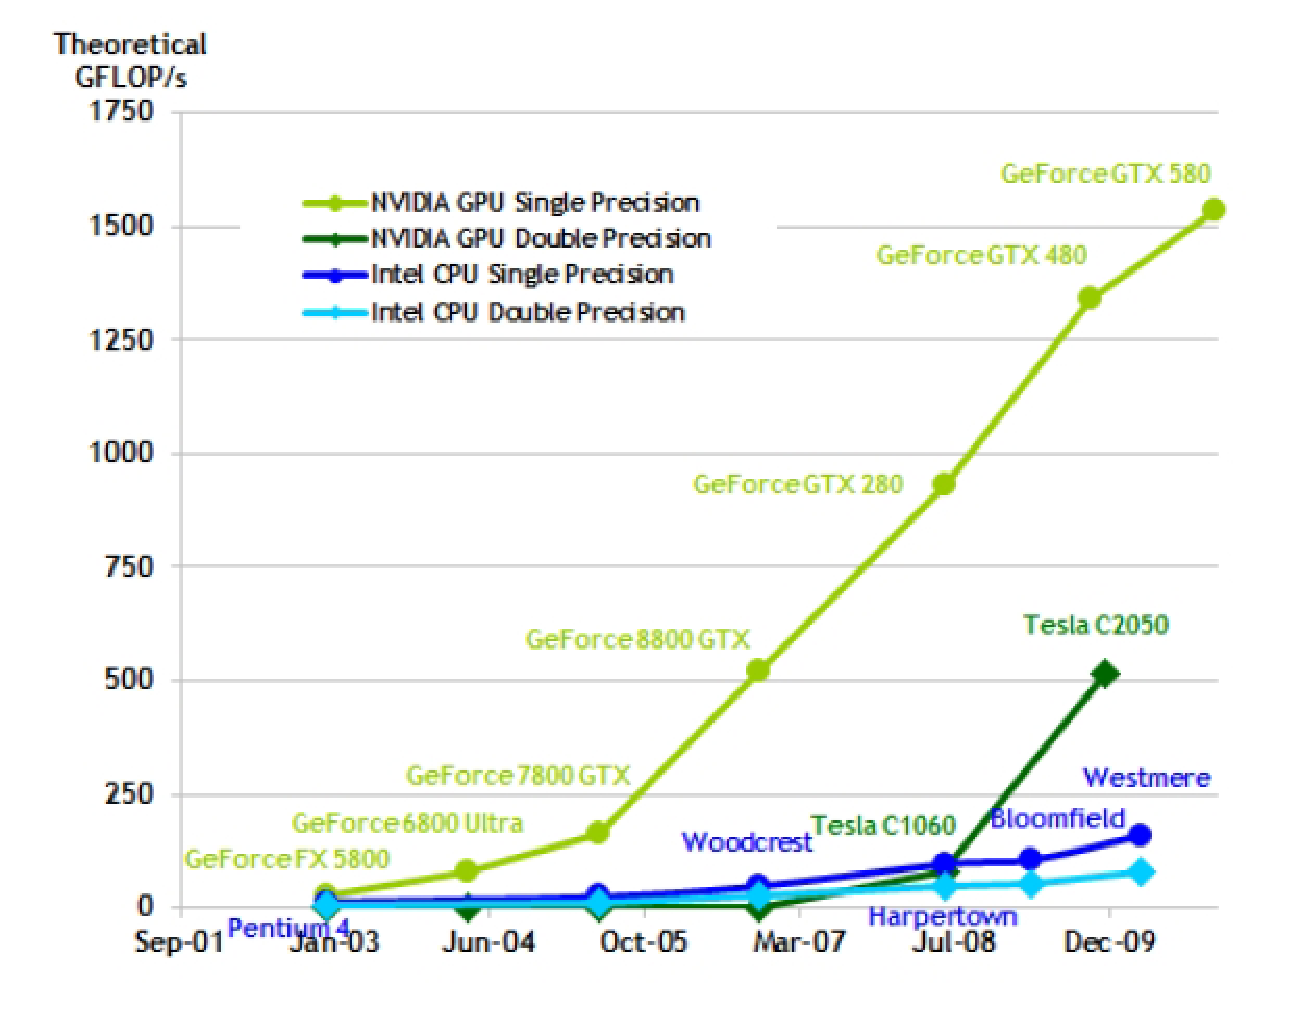
\includegraphics[width=8cm, height=4cm]{./eps/GPU_CPU_chart.eps}
 \caption{CPU vs GPU growth rate in terms of FLoating point Operations Per Second.}
 \label{fig:cpuvsgpu}
\end{figurehere}

Due to its parallel nature, GPU computing can be very effective for applications involving huge amount of data, especially if the data can be represented in sequential structures like vectors and arrays.

\begin{figurehere}
 \centering
 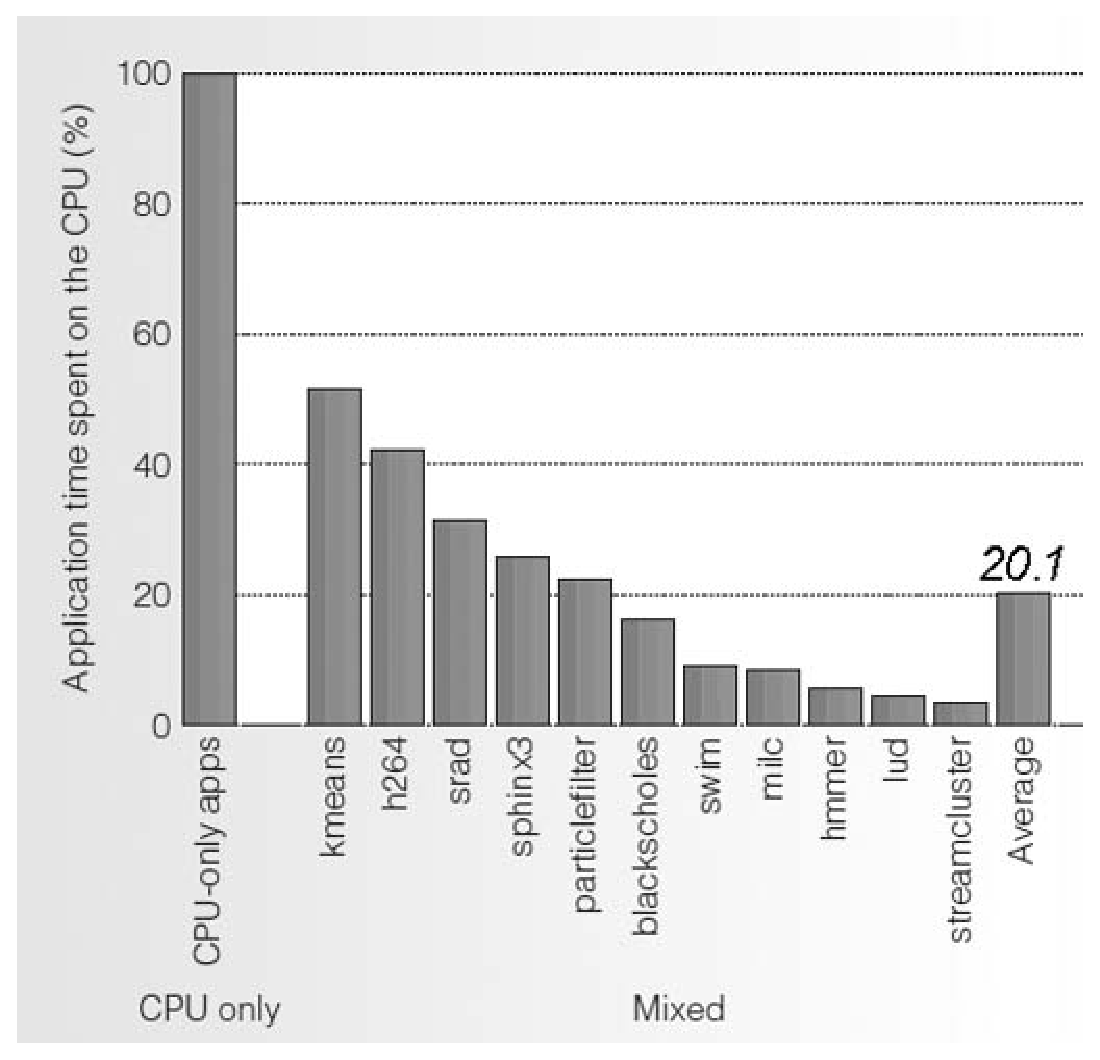
\includegraphics[width=6cm, height=4cm]{./eps/CPU_usage.eps}
 \caption{Time spent on the CPU on various benchmarks using mixed CPU-GPU computation. \cite{Arora:12:Redefining}}
 \label{fig:cpuload}
\end{figurehere}


As you can see in \textbf{Figure \ref{fig:cpuload}}, GPU can offload the CPU from most of its work, but this doesn't mean that CPU performance is no longer critical. Many applications don't (and can't) map all their code to the GPU, and in certain cases the CPU can run some part of the code in a more effective way than the GPU.
Furthermore, not all the code can be mapped easily and clearly on the GPU, as programming GPGPU application can be way more difficult and cryptic than programming in the classical way.

%-----------------------------------------------------------------------------
\subsection{Basic Principles of GPGPU programming} \label{sect:principles}
% Please avoid separations in titles
% and separate text manually

In this section we'll introduce some of the basic principles behind GPGPU programming. Some of these concepts are directly related to the ``graphic-wise'' manner in which the GPU executes its operations, and having a little knowledge of some of the basic concepts of computer graphics can help to understand how GPU computing work and why it is so fast. For instance, GPUs can handle bidimensional matrices natively because that's the natural way to represent textures in memory. On the other hand CPUs designed to to work on single dimension vectors, because that's how the standard RAM is structured.\\
A GPU is basically a \textit{stream processor}\footnote{Stream Processing refers to a SIMD (Single Instruction Multiple Data) paradigm that allows application to exploit (limited) parallel processing over data.}: a single \textbf{kernel} is executed over a stream of data in a monolitic fashion, at a given moment, the same instruction is executed by every computing unit, each one working on a different piece of data.

\subsubsection{Textures = Arrays}
Due to the linear structure of memory, traditional CPUs cannot \emph{physically} create multi-dimensional array, and accessing single rows and columns of a matrix is achieved by offsetting memory addresses of a large linear array. Each one of these ``jump'' in memory translates directly in performance loss.\\
On the other hand, GPUs are architectured to work natively with textures, that are naturally represented in memory by two-dimensional arrays.\\
The ability to work directly over bidimensional (and three-dimensional) memory structures is one of the main reason why GPUs are much more faster than CPUs when it comes to elaborate data.\\
On the other hand, CPUs can handle memory structures much more bigger (and virtually infinite) compared to the those available for the GPU, as many graphic adapters can only work on textures limited in size. The usual maximum size of a texture is usually 2048*2048, or 4096*4096, but modern graphic cards can handle textures of 8192*8192 in size.
The maximum texture size available for a certain graphic adapter can usually be easily retrieved by simple queries made available by the programming API you are using.

\begin{CLCode}
For Example, with OpenCL, you can obtain the maximum supported texture size with the \textsl{clGetDeviceInfo()} function, passing the
\textsl{CL\_DEVICE\_IMAGE2D\_MAX\_WIDTH} and \textsl{CL\_DEVICE\_IMAGE2D\_MAX\_HEIGHT} as parameters.
\end{CLCode}

We will discuss how textures (and \textit{memory objects} in general) are created and accessed in Section \ref{sect:openCLArch}, when we will introduce the OpenCL API.

\subsubsection{Kernels}
If you are familiar with graphic pipeline programming, kernels are the GPGPU equivalent of \textbf{shaders}.\\
Kernel programming is the core concept behind GPU computation and forces the developer to think in a different way as he is used to, as kernels are oriented toward \emph{parallel execution over stream of data}, while standard CPU programming is oriented toward a classical \emph{loop-iterated} implementation.\\
Since the data of our application is stored into multi-dimensional memory objects (the equivalent of a graphical texture), GPU computing basically consists in feeding this memory structures to a kernel that will execute its code over different data elements simultaneously, in the same way that a graphic shader apply the same transformation over multiple pixels to obtain the final image.\\
Once the kernel has finished its computation, the output will be a new memory object that contains the result of the calculation.\\ If we keep in mind that GPUs were born to elaborate graphical data, it will be easier to understand how kernels work and what is the best approach to be taken when it comes to write a GPGPU application.
To understand how this mechanism works, here's an example of a simple graphical shader written in HLSL language that basically scans a texture to find black pixels and turn them to white:

\newpage
{\footnotesize\begin{verbatim}
float3 BlackToWhite(PixelShaderInput input)
{
  if(input.Color.r == 0 &&
	     input.Color.g == 0 && 
     input.Color.b == 0)
     return float3(1,1,1);
  else
     return input.Color;
}
\end{verbatim}}

The same code in a traditional loop-oriented implementation will be something like:

{\footnotesize\begin{verbatim}
void BlackToWhite(float input[4096][4096][3],
                  float output* [4096][4096][3])
{
  for	(int y=0,y<4096,y++)
    for(int x=0;x<4096;x++)
    {
      if(input[x][y][0] == 0 &&
         input[x][y][1] == 0 &&
         input[x][y][2] == 0)
      {
         *output[x][y][0] = 1;
         *output[x][y][1] = 1;
         *output[x][y][2] = 1;
      }
      else
      {
         *output[x][y][0] = input[x][y][0];
         *output[x][y][1] = input[x][y][1];
         *output[x][y][2] = input[x][y][2];
      }
    }
}
\end{verbatim}}


By comparing the two examples, we can note two fundamental things:

\begin{enumerate}
	\item In the shader we do not implement any cycle, the code is iterated \emph{automatically} on every element of the input structure. Also there is no mapping between the input and the output, but only a \textbf{single return}, because the output element is automatically mapped to the same texture coordinate of the input.
	\item Since GPU are meant to work with colors, shaders can natively work on 4 different channels at a time (RGBA), making GPU computation even more versatile and powerful.
\end{enumerate}

While shaders have to be written in low-level specific languages like HLSL or GLSL, kernels take advantage of APIs that allow the programmers to implement and execute them like normal functions. We'll show some examples on how to implement kernels in Section \ref{sect:kernelImplementation}.

\begin{CLCode}
For Example, using the OpenCL API, you can easily create objects of type \textbf{cl\_kernel} and initialize them with the \textbf{clCreateKernel()} function. On page \pageref{sect:kernelImplementation} you can see an example of a kernel function implemented using OpenCL.
\end{CLCode}


\subsubsection{Computation and feedback}
Since GPU's final purpose is to draw something on screen, GPGPU application cannot be simply ``executed'' like traditional ones, and kernels (although they are basically functions) cannot be simply ``called''. To execute a kernel application over the GPU we have to make it think that it is actually drawing something. In GPU computing, ``to execute something'' translates to ``\textit{to draw something}''.
The operations needed for a kernel call (and their shader execution equivalent) are summarized in \textbf{Table \ref{tab:computeVsDraw}}.\\
After the computation has been performed, the result is stored in the target surface.\\

\begin{tablehere}
{\footnotesize
\begin{tabular}{|p{0,3cm}|p{7cm}|}\hline
~ & \textbf{Drawing perspective}\\ \hline
1) & Assign the input texture to a texture channel of the graphic adapter\\ \hline
2) & Set the drawing surface \\ \hline
3) & Define the area to be drawn.\\ \hline
4) & Load the shader\\ \hline
5) & Render the image\\ \hline
~ & ~\\ \hline
~ & \textbf{Computation perspective}\\ \hline
1) & Initialize the input data structure and feed it to the kernel\\ \hline
2) & Define in which memory object the output data will be stored\\ \hline
3) & Initialize the indices and set the bounds of the loop \\ \hline
4) &  ~\\ \hline
5) & Iterate through data and execute the kernel.\\ \hline
\end{tabular}}
  \caption{Drawing and Kernel Execution comparison\\}
	\label{tab:computeVsDraw}
\end{tablehere}

%-----------------------------------------------------------------------------
\subsection{GPGPU APIs and Languages}

In this section we will briefly introduce the most common languages and APIs used to develop GPGPU applications.

\subsubsection{CUDA (www.nvidia.com)} \label{sect:CUDA}
CUDA is the parallel programming platform introduced by Nvidia in 2006 and it has currently reached version 5.
The main focus of CUDA is on parallelism and automatic scalability: the program model forces the programmer to partition the main problem into coarse sub-problems that can be solved independently and in parallel. The various threads are automatically scaled in runtime over the different cores of the GPU, and the developer doesn't have to know in advance the architecture of the graphic adapter. (\textbf{Figure \ref{fig:scalability}}).

\begin{figurehere}
 \centering
 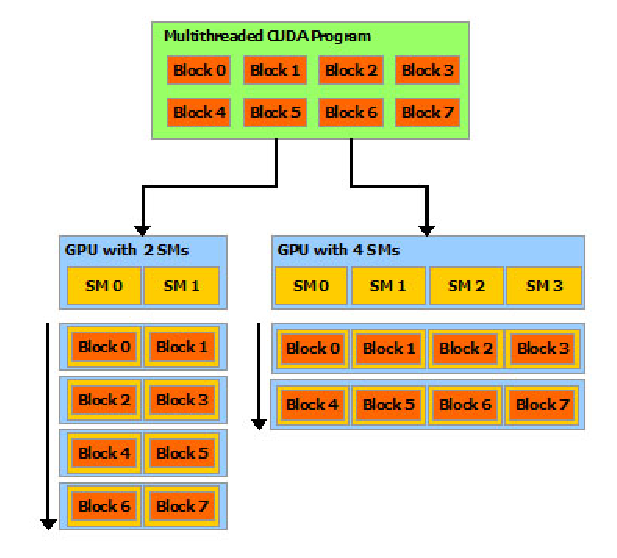
\includegraphics[width=7cm, height=4cm]{./eps/scalability.eps}
 \caption{CUDA executables are automatically scaled over the various SMs (Stream Multiprocessors): a GPU with more multiprocessors will automatically execute the program in less time than a GPU with fewer multiprocessors.}
 \label{fig:scalability}
\end{figurehere}

CUDA is mainly based on C-language and follow the basic principles introduced in Section \ref{sect:principles}, as it uses \textit{Kernels} and texture-like memory structures. It also introduces new concepts like \textbf{thread hierarchy} (allowing to create \textit{multi-dimensional thread blocks} that can be executed in parallel) and \textbf{memory hierarchy} (for example each thread has its own local memory and can share memory with thread in their own block).\\
On the downside, since it is a proprietary framework, CUDA executables will only run on Nvidia graphic cards, and the code cannot fall back on the CPU in the case a CUDA accelerated hardware is not available on the system.\cite{siroro:GPUComparison}

\subsubsection{OpenCL (www.khronos.org/opencl/)}
OpenCL (Open Computing Language) is the parallel programming model developed by the Khronos group that focuses on cross-platforming: differently from CUDA, OpenCL is supported on a wide range of devices and can also be executed on embedded systems and mobile devices.\\
OpenCL applications can also be executed on standard CPUs and don't strictly need to have a graphic adapter installed on the system, this guarantees compatibility with many different devices, especially in the field of embedded systems or non conventional computing.
The current version of OpenCL is 1.2 and we will discuss this parallel programming framework more in deep in Section \ref{sect:openCL}.

\subsubsection{DirectCompute}
Also known as Computer Shader (for more info refer to the msdn library: http://msdn.microsoft.com/), DirectCompute is the GPU computing API developed by Microsoft and it is part of the DirectX APIs collection starting from version 11.
Since it is part of the DirectX package, DirectCompute uses HLSL shading language and integrates well with applications already written with the DirectX API, however, its compatibility is limited to desktop graphic adapters that supports DX10 or 11 and only for Windows (Vista or later) operating systems.

%%%%%%%%%%%%%%%%%%%%%%%%%%%%%%%%%%%%%%%%%%%%%%%%%%%%%%%%%%%%%%%%%%%%%%%%%%%%%